\documentclass{beamer}
\usepackage{xeCJK}
\usepackage{graphicx}
\setCJKmainfont{Noto Serif CJK TC}
%credit to the devs of the metropolis theme
\usetheme{metropolis}

\title{Digital Transformation: Improving the Odds of success}

\author{Andr\'es Ponce(彭思安)}


\institute{National Chiao Tung University}

\begin{document}
\maketitle

\begin{frame}
	\frametitle{Introduction}
	For some select companies, up to 80\% of their revenue comes
	from digital avenues.\pause

	However, making the ``digital transformation" can make the company 
	actually deliver less profit(up to 45\% less).\pause

	What can you do to increase the chances of success when going digital?
\end{frame}

\begin{frame}
	\frametitle{Some things to do}
		\begin{enumerate}
			\item{\textbf{Laying out clear priorities}}\pause
			\item{\textbf{Investing in talent}}\pause
			\item{\textbf{Committing Time and Money}}\pause
			\item{\textbf{Embracing Agility}}\pause
			\item{\textbf{Empowering People}}
		\end{enumerate}
\end{frame}

\section{Laying Out Clear Priorities}
\begin{frame}
	\frametitle{Laying Out Clear Priorities}
	When the executives have a clear vision, there appears
	to be a higher likelihood of success.\pause

	Focus on a few themes/ ideas directly tied to your 
	business\pause

	People need to know what they are working for in order to 
	do it effectively.
\end{frame}

\section{Investing in Talent}
\begin{frame}
	\frametitle{Investing in Talent}
	Sometimes dedicated personnel is required to deal with 
	the digital transformation.\pause

	Most companies that have successfully 
	digitized employ a  Chief Digital Officer(CDO) 
\end{frame}

\section{Committing Time and Money}
\begin{frame}
	\frametitle{Committing Time and Money}
	The company needs to realize that digitizing requires
	commitment -- and not be scared by it.\pause

	Companies that have digitization as one of their top
	priorities were more likely to digitize succesfully.\pause

	Sufficient funds and time need to be allocated.
\end{frame}
\begin{frame}
	\frametitle{Embracing Agility}
	The top digital players are constantly updating their
	digital systems.\pause

	Employees that generate valuable ideas and pursue 
	opportunities should also be rewarded.
\end{frame}
\begin{frame}
	\frametitle{Empowering People}
	Putting people in charge and holding them accountable 
	for their transformation also increases the chance of 
	meeting those goals.\pause

	Create a shared sense of accountability.
\end{frame}
\section{Conclusion}
\begin{frame}
	\frametitle{Conclusion}
	\begin{columns}
	\column{0.4\textwidth}
	Companies can increase the likelihood of digitizing and 
	increasing their profits, regardless of where in the 
	company these changes are applied.
	\column{0.5\textwidth}
		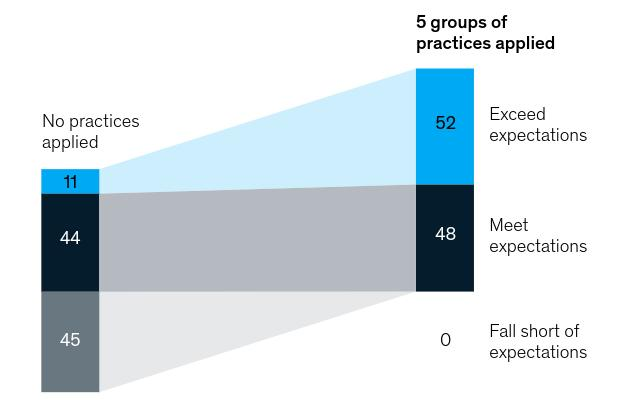
\includegraphics[scale=0.2]{profits}
	\end{columns}
\end{frame}
\end{document}
